\newpage
\section{Suggested solutions: Sinusoidal Signals}
\begin{enumerate}
\item If $x_{\text{noise}}(t)=\cos(\omega t+\phi)$ and $x_{\text{cancel}}(t)=\cos(\omega t+\phi_{c})$ and:
$$x_{\text{noise}}(t)+x_{\text{cancel}}(t)=0,$$
then we must have:
$$\cos(\omega t+\phi)+\cos(\omega t+\phi_{c})=0,$$
for all $t$. The phase doesn't depend on $t$, so it is the same for every $t\in\mathbb{R}$, in particular for $t=0$ so:
\begin{align*}
    \cos(\phi)&=-\cos(\phi_{c}), \\
    \cos(\phi)&=\cos(\pi -\phi_{c}), \\
    \phi+2\pi k&=\pi-\phi_{c}+2\pi l,
\end{align*}
for $k,l\in\mathbb{Z}$, which gives $\phi_{c}=\pi-\phi+2\pi(l-k)=\pi-\phi+2\pi m$, 
where $m\in\mathbb{Z}$. Take $m=0$ to obtain a simple solution, which gives $\phi_{c}=\pi -\phi$.
Hence, the canceling signal must be of the form:
$$x_{\text{cancel}}(t)=\cos(\omega t+(\pi-\phi)).$$
A simple test program to verify this is shown in Listing \ref{cancel} 
with an arbitrary choice of $\omega$, $\phi$ and $m$. 
If the code is run, two signals of opposite amplitude are shown, 
which cancel out when added, as hoped. 
\lstinputlisting[language=Python,caption={Noise canceling signal},label=cancel,linerange={0-25}]{ch06/code/ex6.1.py}

\item Have that:
$$a\cos(\omega t)+b\sin(\omega t)=\frac{a}{2}(e^{i\omega t}+e^{-i\omega t})+\frac{b}{2i}(e^{i\omega t}-e^{-i\omega t}),$$
or written out:
$$a\cos(\omega t)+b\sin(\omega t)=\frac{a}{2}e^{i\omega t}+\frac{a}{2}e^{-i\omega t}+\frac{b}{2i}e^{i\omega t}-\frac{b}{2i}e^{-i\omega t}.$$
Using the phasor summation property we have:
$$X=\sum_{n}X_{n}=\frac{a}{2}+\frac{b}{2i}=\frac{1}{2}(a-bi),$$
and
$$Y=\sum_{m}Y_{m}=\frac{a}{2}-\frac{b}{2i}=\frac{1}{2}(a+bi).$$
Then we have that:
\begin{align*}
    |X|&=\sqrt{\frac{1}{4}(a^{2}+b^{2})}=\frac{1}{2}\sqrt{a^{2}+b^{2}}, \\
    |Y|&=\sqrt{\frac{1}{4}(a^{2}+b^{2})}=\frac{1}{2}\sqrt{a^{2}+b^{2}},
\end{align*}
and
\begin{align*}
    \angle X&=\arctan\left(\frac{-b}{a}\right)=\phi, \\
    \angle Y&=\arctan\left(\frac{b}{a}\right).
\end{align*}
Then the whole expression can be rewritten as:
\begin{align*}
    a\cos(\omega t)+b\sin(\omega t)&=\frac{1}{2}\sqrt{a^{2}+b^{2}}e^{i\phi}e^{i\omega t}+\frac{1}{2}\sqrt{a^{2}+b^{2}}e^{-i\phi}e^{-i\omega t}, \\
    &=\frac{1}{2}\sqrt{a^{2}+b^{2}}e^{i(\omega t+\phi)}+\frac{1}{2}\sqrt{a^{2}+b^{2}}e^{-i(\omega t+\phi)}, \\
    &=\sqrt{a^{2}+b^{2}}\left[\frac{1}{2}\left(e^{i(\omega t+\phi)}+e^{-i(\omega t+\phi)}\right)\right], \\
    &=\sqrt{a^{2}+b^{2}}\cos(\omega t+\phi), \\
    &=A\cos(\omega t+\phi).
\end{align*}
Here $A=\sqrt{a^{2}+b^{2}}$ and $\phi=-\arctan(b/a)$, where $\arctan(b/a)$ 
should give the angle corresponding to which quadrant the point $(a,b)$ lies in the $xy$-plane. 

\item Consider the signal:
$$x(t)=\cos(\omega_{1}t)\sin(\omega_{2}t),$$
which we can write as:
$$x(t)=\frac{1}{2}(e^{i\omega_{1}t}+e^{-i\omega_{1} t})\frac{1}{2i}(e^{i\omega_{2}t}-e^{-i\omega_{2}t})=\frac{1}{4i}[e^{i(\omega_{1}+\omega_{2})t}-e^{i(\omega_{1}-\omega_{2})t}+e^{i(-\omega_{1}+\omega_{2})t}-e^{i(-\omega_{1}-\omega_{2})t}].$$
Collecting terms we get:
\begin{align*}
    x(t)&=\frac{1}{4i}[e^{i(\omega_{1}+\omega_{2})t}-e^{-i(\omega_{1}+\omega_{2})t}]+\frac{1}{4i}[e^{i(-\omega_{1}+\omega_{2})t}-e^{-i(-\omega_{1}+\omega_{2})t}], \\
    &=\frac{1}{2}\sin((\omega_{1}+\omega_{2})t)+\frac{1}{2}\sin((\omega_{2}-\omega_{1})t).
\end{align*}
This yields the values $a=1/2$ and $b=1/2$, while $\omega_{3}=\omega_{1}+\omega_{2}$ and $\omega_{4}=\omega_{2}-\omega_{1}$. 

\item The plane wave:
$$E(x,t)=E_{0}e^{i(kx+\omega t)}\partial_{y}$$
is a solution to the wave equation. Consider the real part $\Re\{E(x,t)\}$:
$$\Re\{E(x,t)\}=\frac{1}{2}[E(x,t)+E^{*}(x,t)]=\frac{1}{2}E_{0}(e^{i(kx+\omega t)}+e^{-i(kx+\omega t)})\partial_{y}=E_{0}\cos(kx+\omega t)\partial_{y}.$$
Recall that the wave equation is:
$$\partial_{t}^{2}E-\frac{1}{\mu_{0}\epsilon_{0}}\nabla^{2}E=0,$$
which gives:
$$-\omega^{2}E_{0}\cos(kx+\omega t)\partial_{y}+\frac{1}{\mu_{0}\epsilon_{0}}k^{2}E_{0}\cos(kx+\omega t)\partial_{y}=E_{0}\left(\frac{1}{\mu_{0}\epsilon_{0}}k^{2}-\omega^{2}\right)\cos(kx+\omega t)\partial_{y}=0,$$
since $k^{2}c^{2}-\omega^{2}=0$, as $c=\sqrt{1/\mu_0\epsilon_0}$. In conclusion, the signal:
$$\Re\{E(x,t)\}=E_{0}\cos(kx+\omega t)\partial_{y},$$
is a solution to the wave equation. 

\item If we have an arbitrary number of solutions to the wave equation, each with different 
phasors $E_{n}$ and different angular frequencies $\omega_{n}$. Then a superposition:
$$E(x,t)=\sum_{n}E_{n}e^{i(\omega_{n}/c)x}e^{i\omega_{n}t}\partial_{y},$$
is also a solution. This follows by the linearity of the wave equation. 

\item The code from the notes has been modified such that the output signal has a frequency of approximately 42.0 Hz. 
\lstinputlisting[language=Python,caption={Adding frequencies},label=sig42,linerange={0-35}]{ch06/code/ex6.6.py}
Running the code in Listing \ref{sig42} yields the following output:
\begin{figure}[h!]
    \centering
    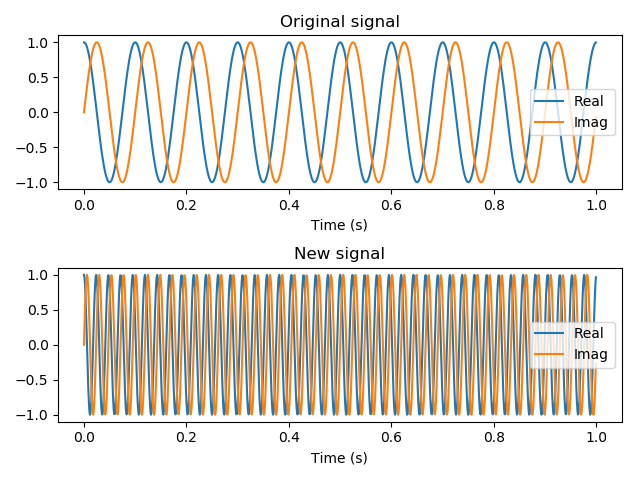
\includegraphics[scale=1.0]{ch06/figures/ex6a.png}
    \caption{Signal with 42 Hz frequency}
\end{figure}

\item The following code is a modification that multiplies the signal with a periodic 5.0 Hz signal:
\begin{itemize}
\item[a)] Listing \ref{sig42_mod} provides a suggested solution.
\lstinputlisting[language=Python,caption={Modifying signals},label=sig42_mod,linerange={0-22}]{ch06/code/ex6.7a.py}
Running Listing \ref{sig42_mod} produces Figure \ref{fig:ex6b}.
\begin{figure}[h!]
    \centering
    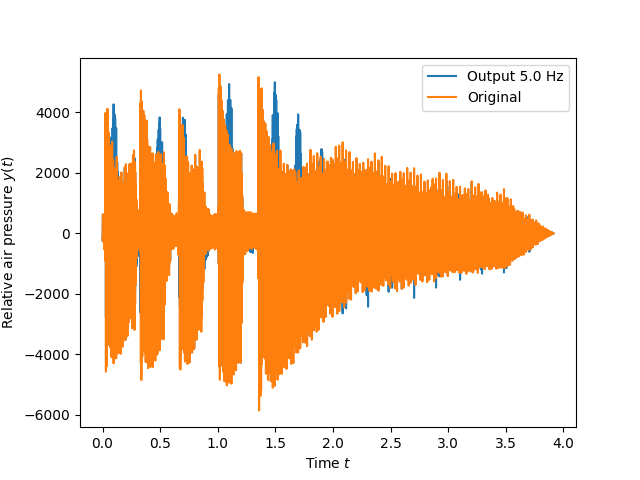
\includegraphics[width=12.5cm,height=9.5cm]{ch06/figures/ex6b.png}
    \caption{Original and modified guitar signal}
    \label{fig:ex6b}
\end{figure}

\item[b)]
Adding the following code to Listing \ref{sig42_mod} will save the result as an audio file.
\begin{lstlisting}[language=Python,caption=Saving an audiofile,label=save_audio]
out = 0.9*out/n.max(n.abs(out)) 
# write compressed output to wav file.

# multiply the signals
out2 = x*n.cos(2.0*n.pi*time_vec*2.5)

sio.write("guitar_leslie.wav",sample_rate,n.array(out,dtype=n.float32))
\end{lstlisting}
Listening to the audio file, we hear that the guitar sound has a wavy oscillating effect.

\item[c)]
Based on the previous task, the result of multiplying with a 2.5 Hz signal will result in the same effect, but the oscillation will be slower. 
After testing this by running Listing \ref{save_audio} this is exactly what happens. 
\end{itemize}




\end{enumerate}
